% Use with graphicx. PNG files are immediately usable; SVGs are supplied
% for journal production. Paths are relative to this R09 fragment.
\begin{figure}[ht]
 \centering
 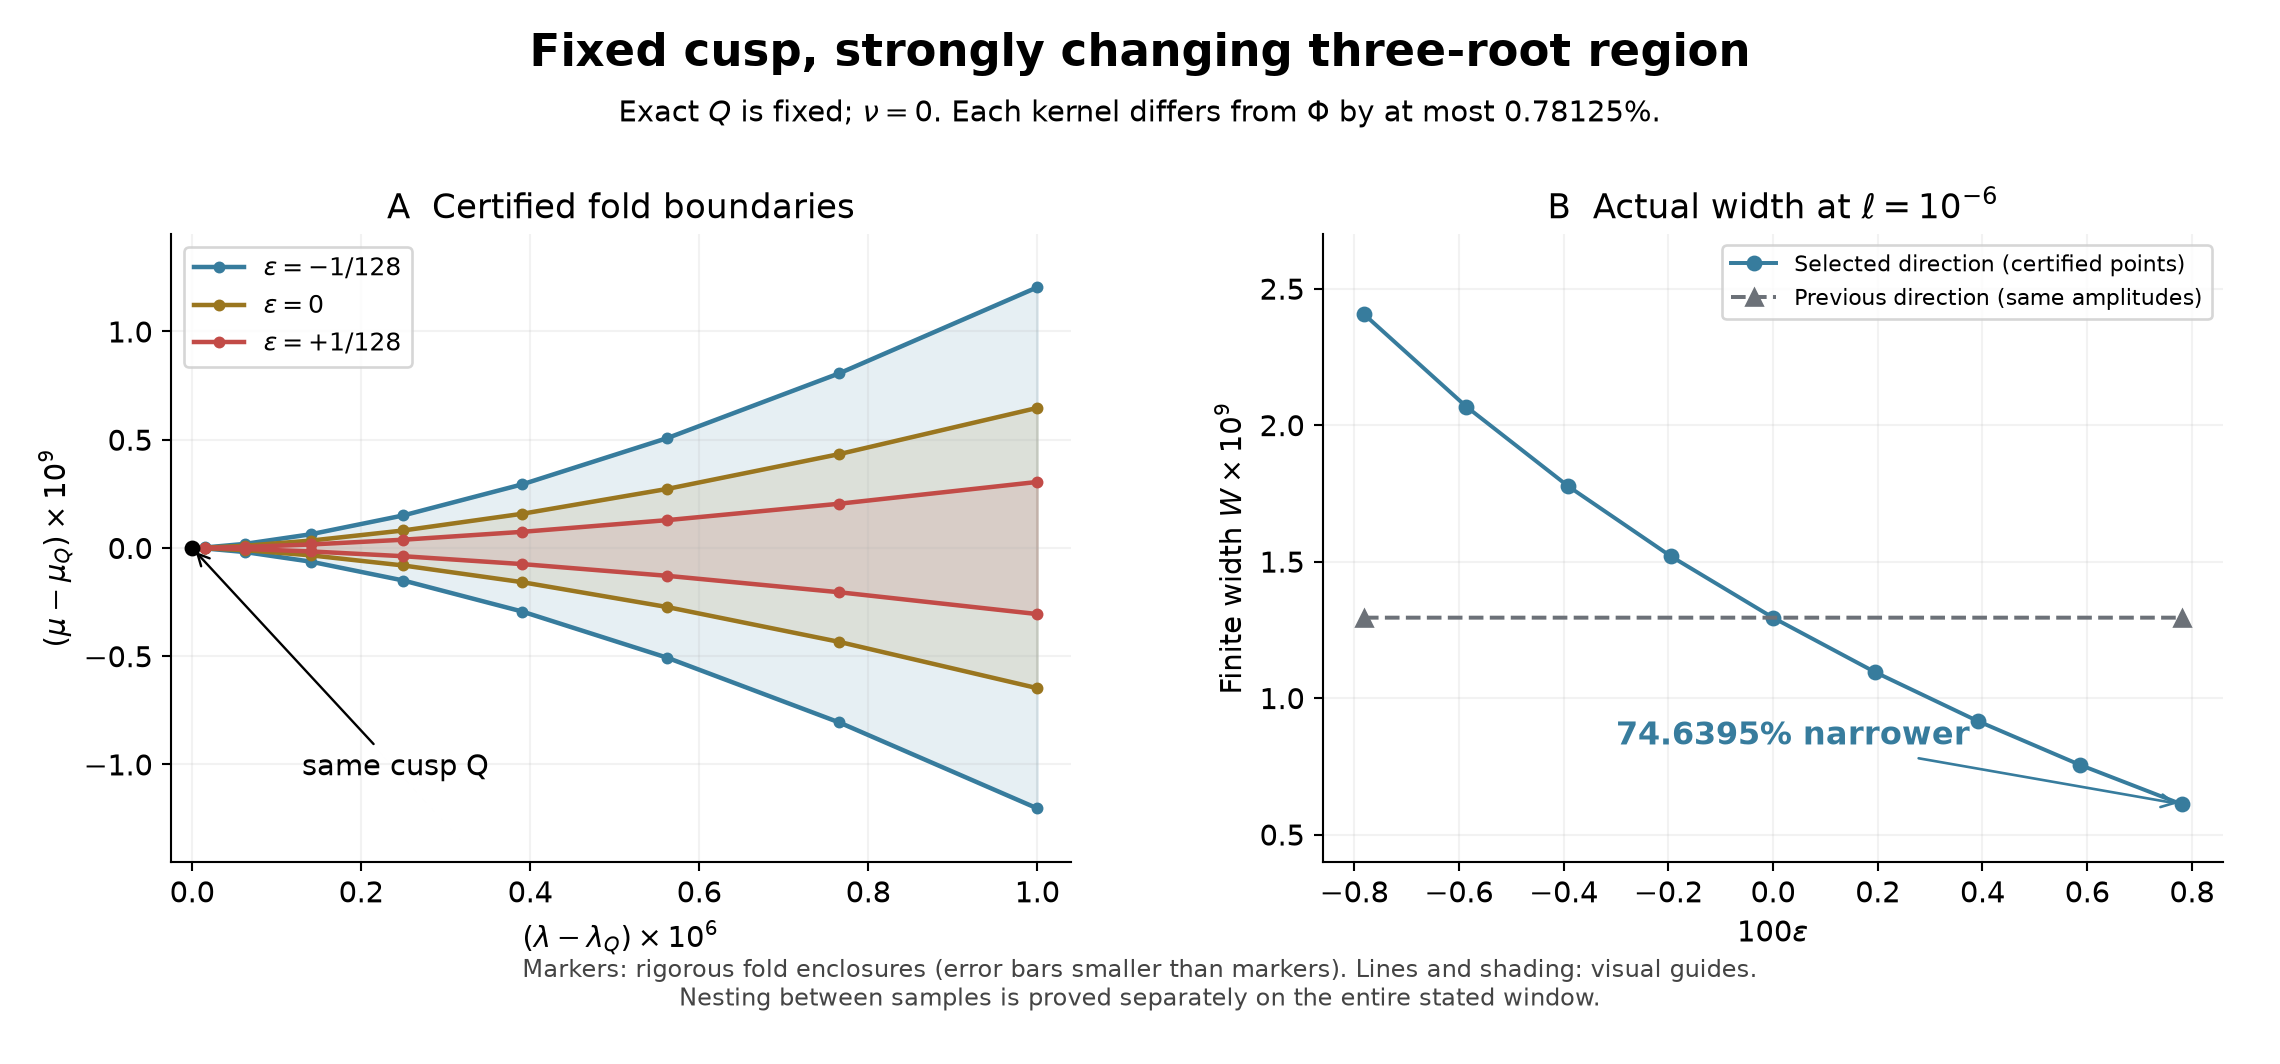
\includegraphics[width=\textwidth]{figures/finite_shape_design.png}
 \caption{Finite geometric change at the exact pinned cusp $Q$, with
 $\nu=0$. Left: the two fold boundaries for three amplitudes of the
 selected direction; the intervening region has three simple real
 zeros in the certified $t$ window. Right: the actual fold width at
 $\ell=10^{-6}$, compared with the earlier direction at the same
 endpoint amplitudes. Each displayed kernel differs from the base
 kernel by at most $0.78125\%$ pointwise. Markers are rigorous fold
 enclosures; their widths are smaller than the markers. Connecting
 lines and shading are visual guides. Continuum nesting between
 the samples is established separately by the amplitude-cell proof.}
\end{figure}

\begin{figure}[ht]
 \centering
 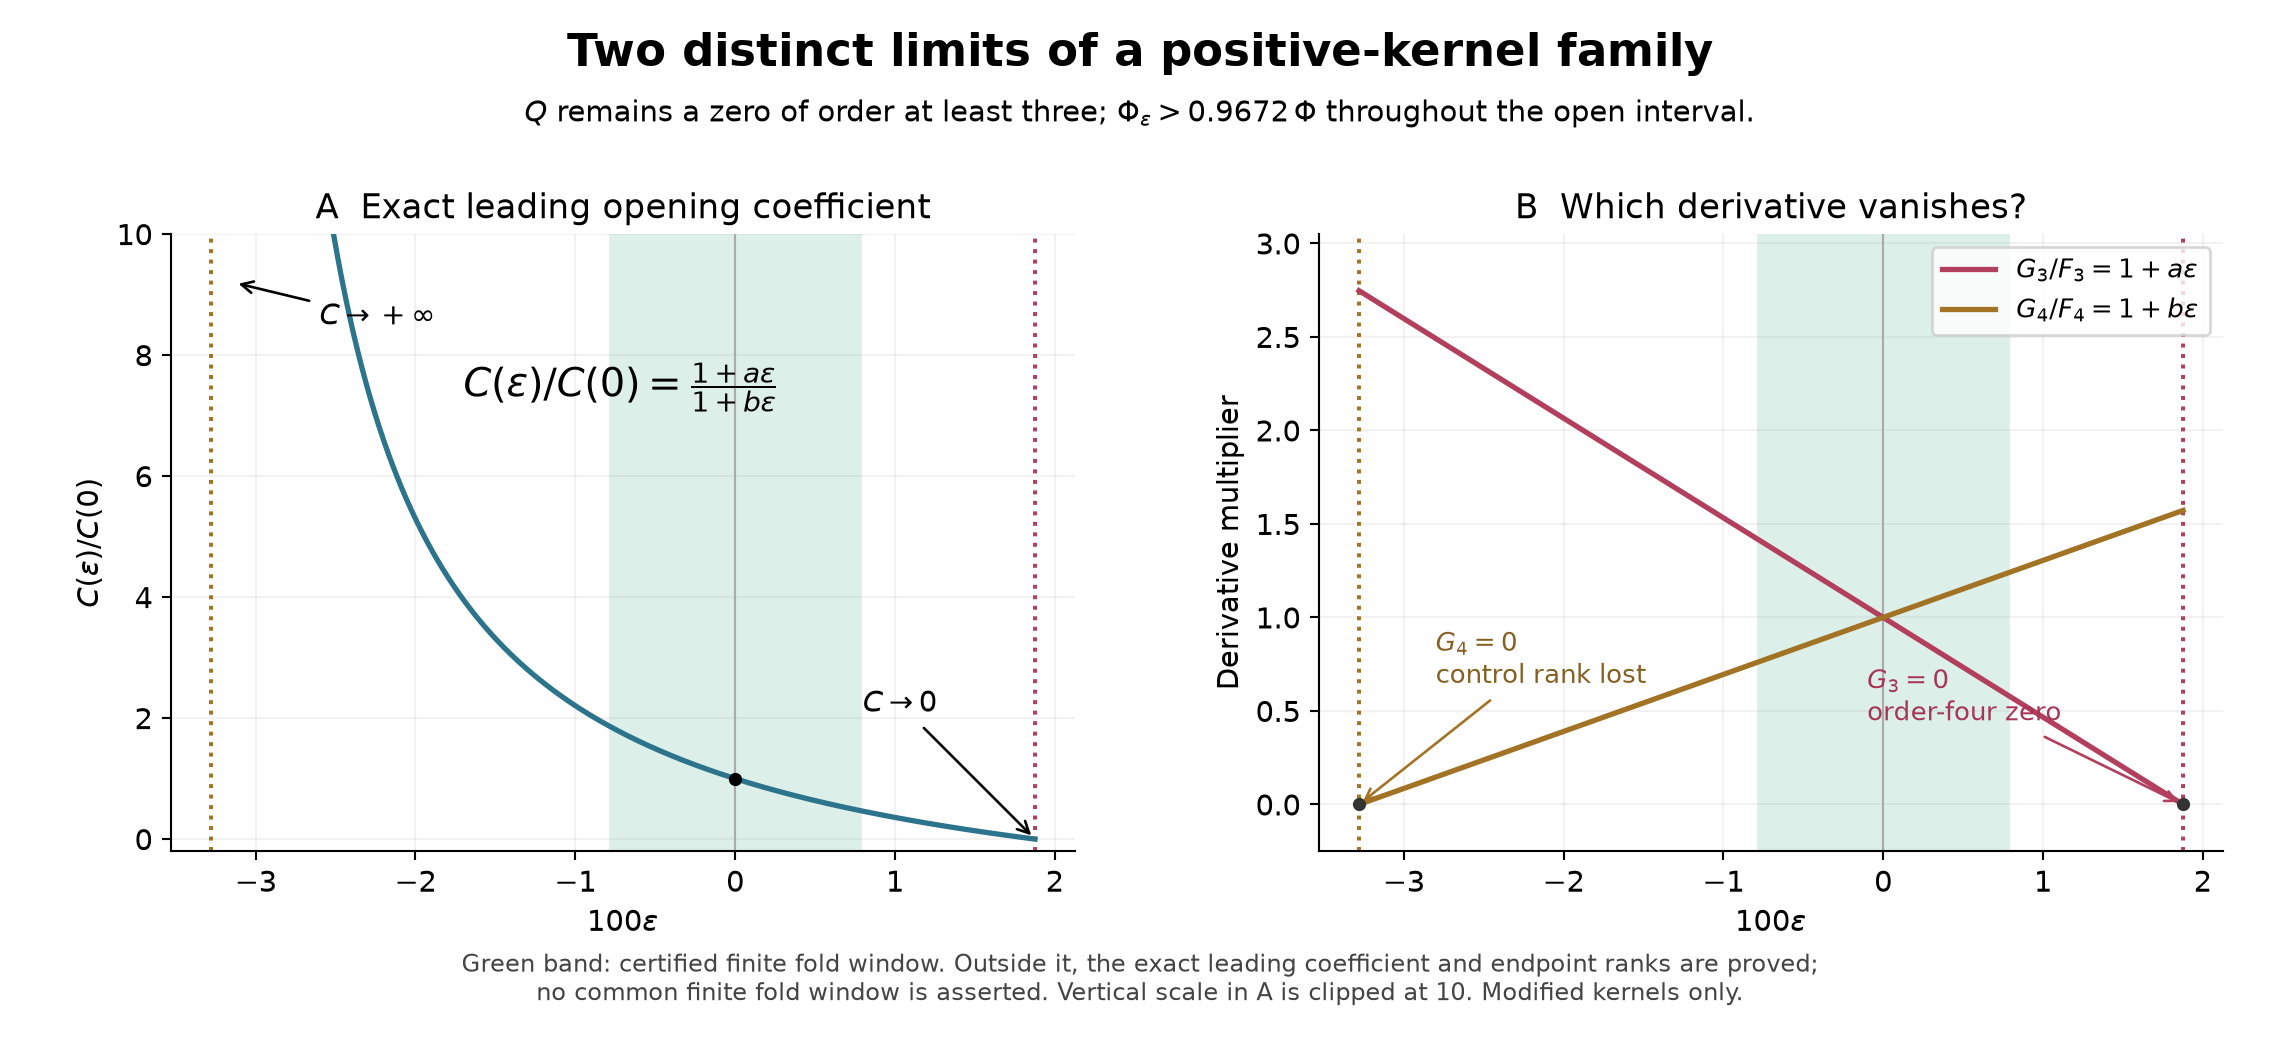
\includegraphics[width=\textwidth]{figures/opening_boundaries.png}
 \caption{Exact leading opening and two distinct endpoint mechanisms
 for the selected positive-kernel family. Left:
 $C(\epsilon)/C(0)=(1+a\epsilon)/(1+b\epsilon)$; the vertical scale
 is clipped at 10. Right: normalized third and fourth $t$ derivatives
 at the fixed $Q$. At the negative endpoint the $(\lambda,\mu)$
 cusp unfolding loses rank while the root remains third order.
 At the positive endpoint the root has order four and the three-control
 jet matrix has full rank. The green band denotes the amplitudes
 for which the common finite fold window is certified. Outside it,
 this figure concerns the leading coefficient, not a certified
 finite width on a common window. All kernels here are modified
 kernels; the original fixed-kernel family is a distinct scope.}
\end{figure}
